\section{Introduction}
\subsection{Data wrangling is data analysis}

Data analysis is not simply implementing statistical analyses. Data analysis is an iterative process including data collection, clean-up (tidying), transformation in and between data sets,  visualization, and statistical analysis, see \ref{fig:data_wrangling} \parencite{Wickham2017R}. Yet, all too often quantitative multilingual research reports vague practices or fails to report any decisions made during data analysis process outside of statistical models, in part, because pre-processing software has already made the decisions for the researchers \parencite{Prystauka_Altmann_Rothman_2023}. Wrangling decisions have pervasive implications across data analysis that affect replicability and reliability \parencite{ana_flex}. This is especially true for online research implementing methods that capture real-time language processing, such as eye-tracking and mouse-tracking. Whereas open research practices, including shared data and code \parencite{Bolibaugh}, certainly serve as a positive first step, the field still has a long way to go. 

\begin{figure}[h]
    \centering
    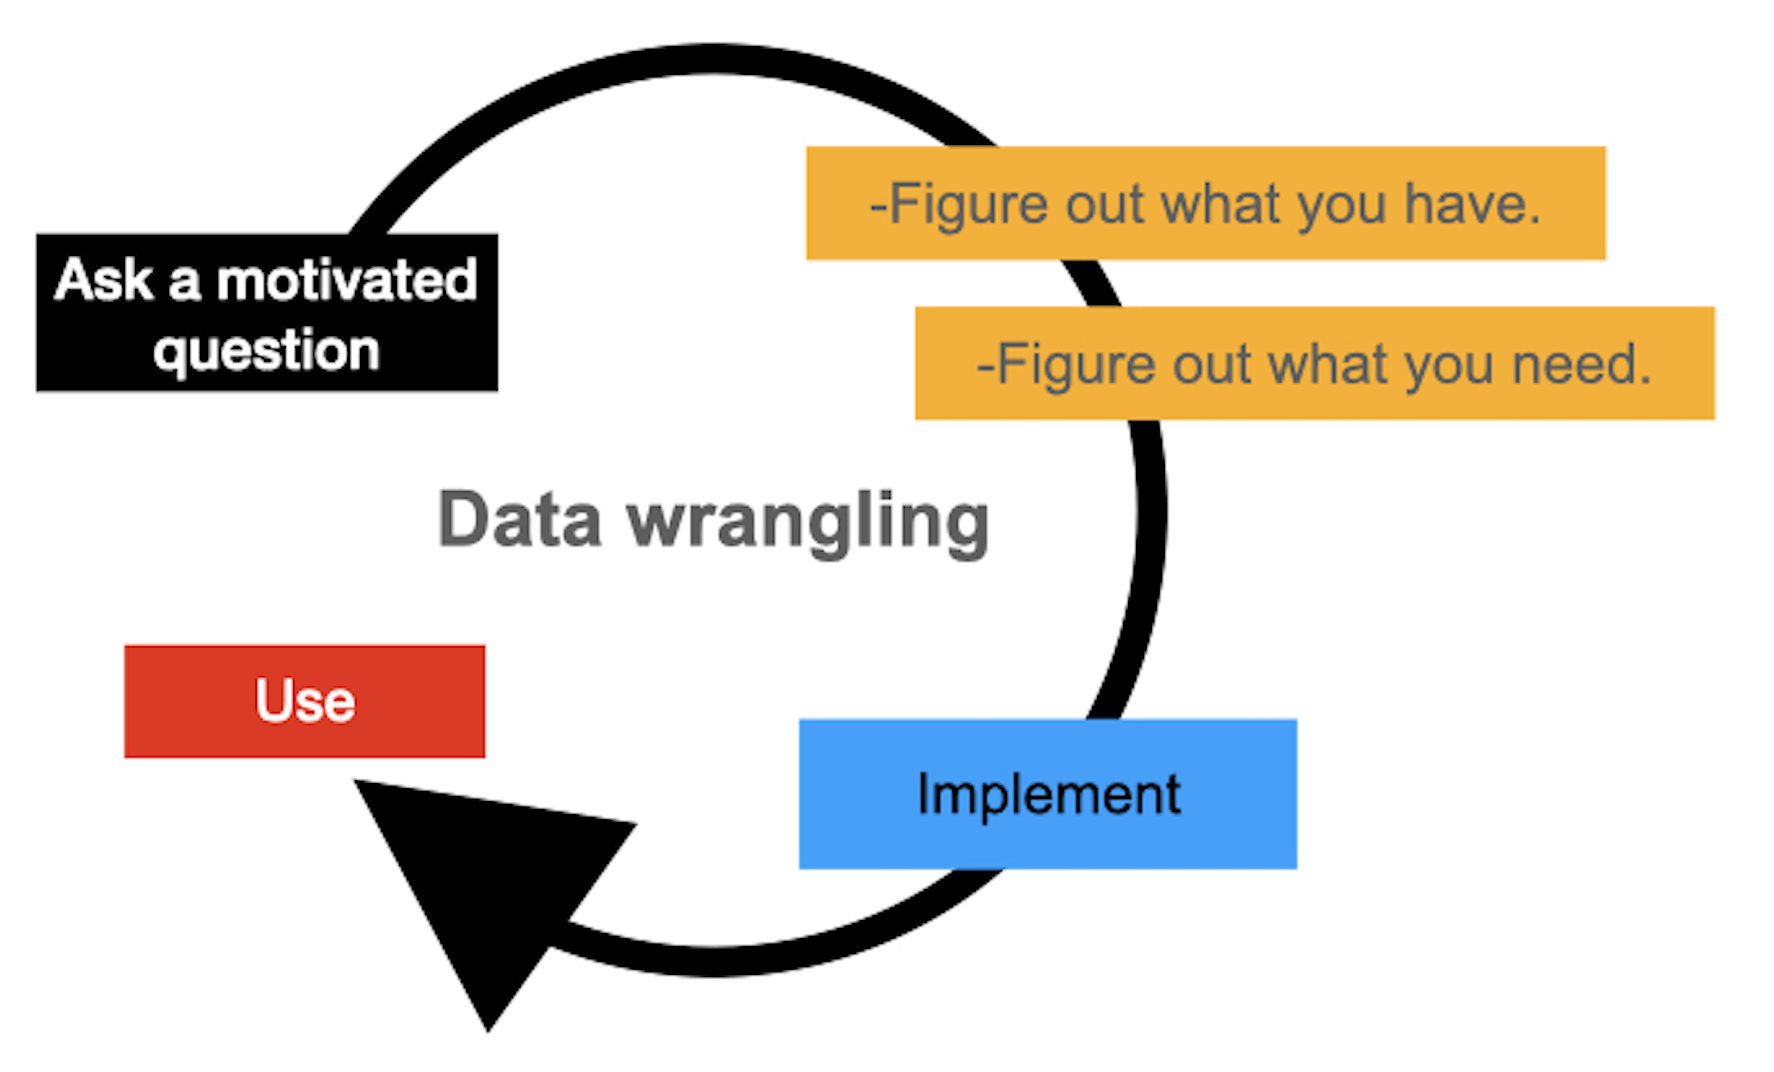
\includegraphics[width=\textwidth]{figures/data_wrangling.png}
    \caption{The data wrangling cycle: the iterative process of data wrangling, includes all steps, which reduce, reorder, extend, tidy, transform, and/or combine your data}
    \label{fig:data_wrangling}
\end{figure}

Here, we focus on the data wrangling processes of cleaning raw data straight from an experiment and transforming it into a usable structure (i.e., tidy data or data ready for visualization and statistical analysis) within a typical visual world paradigm eye-tracking study.  Web-based eye-tracking and mouse tracking have become more accessible and reliable than ever, capturing many effects found in in-person real-time processing experiments for a fraction of the cost \parencite[e.g.,][]{Vos_2017,Semmelmann_2017,Prystauka_Altmann_Rothman_2023,Degen_Seeing_2021}. However, access to these methods comes at the cost of requiring expertise in data wrangling \parencite[e.g., ][]{Vos_2017,Prystauka_Altmann_Rothman_2023}. Data from online experiments are currently even more complex than their in-person counterparts given the lack of subscriber based pre-processing software, which means that the choices made during data wrangling are a new opportunity for radical open science practices. We present the Art of wrangling as a toolkit which allows the researcher to be prepared and equipped for the most common ways to refine, restructure, and map raw data into a usable format using the lingua franca of data analytics, R \parencite{mizumoto_r_2015}. These tools are not limited to preparing data for analysis or visualization but rather essential for exploring and understanding data itself throughout the data analysis process. 
